\chapter{Introducción}
Con la demanda incremental de aplicaciones, tanto para el entretenimiento 
como para el estudio biomédico, la información visual cada vez tiene un rol 
más importante. Sin embargo, la calidad de la información puede sufrir drásticamente
con las etapas de adquisición, procesado, compresión, transmisión y reproducción.
Es por ello que poder evaluar la calidad de la información se ha vuelto un 
tema cada vez más importante\cite{VisualMedicalQualityBook}.
\section{Definición del Problema}   
La evaluación de la calidad de la imagen (\emph{IQA}) es un problema fundamental 
en el procesamiento de imágenes y de visión por computador. Se refiere a la 
tarea de medir y cuantificar la calidad perceptual de una imagen, 
teniendo en cuenta factores como el contenido, la resolución, 
el contraste, las distorsiones visuales y la percepción humana. 
La mejora de las técnicas suele estar altamente conectado con el avance 
de los estudio del sistema de visión humano (\emph{HVS})\cite{Wang2006ModernIQ}.
 
El problema de la evaluación de la calidad de la imagen se aborda mediante enfoques 
subjetivos y objetivos. Los enfoques subjetivos implican realizar experimentos 
perceptuales en los que se recopilan las opiniones y evaluaciones de los observadores 
humanos. Estos observadores pueden calificar las imágenes en términos de su 
calidad visual o realizar comparaciones entre diferentes versiones de una misma imagen. 
Con base a las respuestas recopiladas, se pueden establecer modelos y 
métricas que reflejen la calidad percibida por los humanos, también conocida
como \emph{MOS}\footnotemark[1].

Alternativamente, los enfoques objetivos buscan desarrollar algoritmos y métricas 
automáticas que puedan estimar la calidad de la imagen sin intervención humana. 
Estos enfoques se basan en características y propiedades visuales extraídas de la 
imagen, que se utilizan para calcular una puntuación de calidad. Estas características 
pueden incluir medidas de nitidez, contraste, estructura, color, distribución de 
texturas y otros aspectos relevantes para la percepción visual.
 
La elección entre enfoques subjetivos u objetivos depende del contexto y los 
recursos disponibles. Los enfoques subjetivos son considerados como la referencia estándar 
para la evaluación de la calidad de la imagen, ya que capturan la apreciación 
humana. Sin embargo, estos enfoques pueden ser costosos y requieren de un número 
significativo de participantes. 
Mientras que, los enfoques objetivos se pueden llegar a automatizar. Haciendo que 
sea muy prácticos para grandes cantidades de datos y diversas aplicaciones.
 
No obstante, el objetivo es desarrollar algoritmos y métricas que puedan proporcionar una 
estimación precisa y consistente de la calidad de la imagen, teniendo en cuenta
tanto aspectos subjetivos como objetivos respecto a las distorsiones.
Para así poder evaluar y comparar diferentes métodos de adquisición, compresión, 
restauración o manipulación de imágenes teniendo en cuenta que el receptor 
final es el humano.
 
Para abordar el problema de la IQA, se emplean diversas técnicas y enfoques. 
Entre ellos se incluyen métodos basados en características de baja y alta calidad,
modelos de percepción visual, aprendizaje automático y técnicas de procesamiento de señales
 
Uno de los enfoques comunes es utilizar características básicas de la imagen. 
Las características elementales de la imagen son por ejemplo el contraste, 
la nitidez, la exposición y la uniformidad del color~\cite{Wang2006ModernIQ} . 
Estas características pueden ser cuantificadas mediante algoritmos de procesamiento de 
imágenes y proporcionar una estimación inicial de la calidad. 
 
Por otro lado, los modelos de percepción visual intentan simular cómo el sistema 
visual humano percibe y evalúa la calidad de la imagen. Estos modelos se basan 
en el entendimiento de los mecanismos y procesos perceptuales del cerebro humano, 
y utilizan características visuales y estadísticas para calcular la calidad percibida
\cite{MinkowskiFailure, StructuralSimilarityIndex}.
Estos modelos buscan emular la forma en que los humanos interpretan y responden 
a las imágenes en términos de su calidad visual\cite{IQAbySaliencyMaps, CascadedIQA}.
 
Habitualmente, se suelen emplear algoritmos de aprendizaje automático para tratar
de resolver el problema. Se utilizan técnicas supervisadas o no supervisadas 
para intentar aproximar una función que a partir del conjunto de características 
extraídas pueda determinar la calidad de la imagen en una escala específica, 
generalmente en el rango de 0 a 10.

\footnotetext[1]{\emph{Mean Opinion Score} o Valor medio de opinión, consiste en 
la media de la opinión de diversas personas para establecer un valor de referencia. }

\subsection{Subproblemas y dificultades}
Existen tres subproblemas presenten en el ámbito de \emph{IQA}. Los primeros, son problemas 
dónde tenemos acceso a la imagen original, que suponemos exenta de desperfectos, 
en la cúal se pueden aplicar métodos basados en diferencia de características 
entre ambas, como puede ser al nivel del color de píxel posición a posición,
y se denomina ``\emph{Full Reference}''(\emph{FR}). 
La tarea, aparentemente sencilla, en realidad presenta una complejidad alta dada por 
la necesidad de codificar la percepción humana a la hora de calificar la calidad 
de una imagen\cite{WhyIsIQASoDifficult}. Ya que métricas que miden distancias no suelen ser suficientes, 
ver imágenes~(\ref{fig:FailureMinkowskiMetric},\ref{fig:MSEHyperSphere}).
 
Los segundos son aquellos dónde tenemos algún tipo de información adicional respecto 
a la imagen original en el momento de asesoramiento de la calidad de la imagen final,
denominados ``\emph{Reduced Reference}''(\emph{RR}). La información extra puede incluir características estadísticas, metadatos, parámetros 
de compresión o características extraídas de una región de interés específica.
 
Y por último, tenemos aquellos problemas donde desconocemos el origen y cualquier 
información respecto a la imagen inicial, denominados problemas ``\emph{No reference}''(\emph{NR}).
Estas métricas están exentas de cualquier información de referencia y se 
centran en capturar características generales de calidad. 

La complejidad del problema crece conforme nos desplazamos a las tres dimensiones. 
El asesorar la calidad de los modelos \emph{3D} implica mayor nivel de dificultad 
dado que nos enfrentamos a dos grandes retos: La complejidad computacional 
de las operaciones y la escasez de bases de datos etiquetadas
sobre objetos tridimensionales para entrenar y evaluar modelos. 
 
Para las nubes de puntos, que representan una colección de puntos en un espacio 
tridimensional $(x,y,z)$ cada uno con un color asociado \emph{RGB}, se pueden emplear métricas y algoritmos basándose en criterios como la 
densidad de puntos, la uniformidad, la precisión geométrica y la detección de artefactos.
También se pueden considerar aspectos relacionados con la coherencia de los colores 
o texturas asociadas a los puntos\cite{NR3DQA, StructureGuidedResampling, GPA-NET} 
 
Un enfoque común es la evaluación de calidad de una nube de puntos tridimensional 
mediante proyecciones \emph{2D} desde diferentes perspectivas\cite{IT-PCQA, VQA-PC, MM-PCQA}. 
De esta forma podemos tratar el problema como uno de \emph{IQA} reduciendo la 
complejidad computacional, pudiendo implementar métodos y soluciones ya existentes.

Teniendo en cuenta todas estas consideraciones, el presente TFG aborda la
estimación de calidad de imágenes médicas en espacio tridimensional.

\begin{figure}[htp]
  \begin{center}
    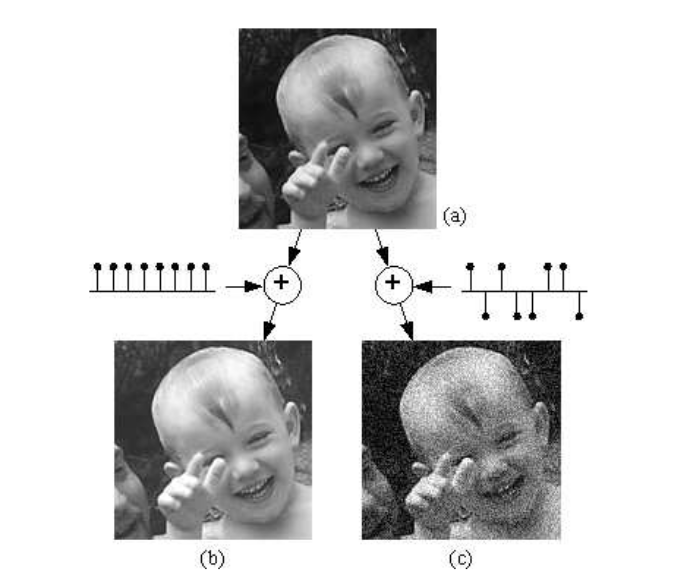
\includegraphics[width=0.5\textwidth]{imagenes/Chapter1/failure_minkowski_metric.png}
  \end{center}
  \caption{En este ejemplo, extraído de\cite{MinkowskiFailure},
  vemos que sumar una constante positiva a una imagen  de referencia (a) produce la imagen (b) que contiene la misma distancia \emph{Minkowski}\footnotemark[1]
  que (c), imagen fabricada por la misma constante pero permutando signo de forma aleatoria. Siendo que
  la percepción final es que la imagen (c) es peor que la (b).
\label{fig:FailureMinkowskiMetric}}
\end{figure}
\begin{figure}[htp]
  \begin{center}
    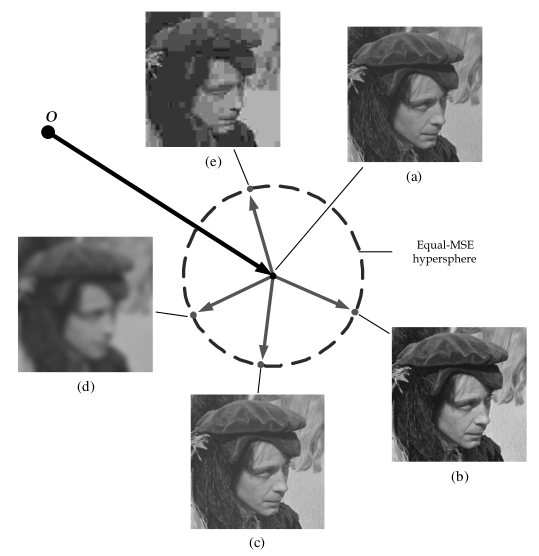
\includegraphics[width=0.5\textwidth]{imagenes/Chapter1/MSE_Hypersphere.png}
  \end{center}
  \caption{En este ejemplo, extraído de\cite{Wang2006ModernIQ} la misma imagen distorsionada de distintas maneras
  resulta en el mismo valor \emph{MSE}\footnotemark[2]=181. Siendo evidente que 
  algunas distorsiones producen efectos visuales más marcados que otras haciendo 
  que no sea una buena estimación perceptual de la calidad.}
  \label{fig:MSEHyperSphere}
\end{figure}

\footnotetext[1]{La distancia de \emph{Minkowski} es una métrica 
vectorial que puede considerarse como una generalización tanto de 
la distancia euclidia como de la distancia de Manhattan . }
\footnotetext[2]{\emph{MSE}: \emph{Mean squared error} o error cuadrático medio 
  es una métrica de distancia que se calcula como la media de la suma de las 
  diferencias al cuadrado.}

\section{Motivación}
 
En el caso del ámbito biomédico, dado los rápidos avances en las últimas década
de las técnicas no invasivas de imágenes y la gran cantidad de fabricantes 
de equipamentos, nació el estándar \emph{DICOM}~\cite{Parisot1995} en 1995 
con objetivo de hacer que el intercambio de imágenes médicas se realice de forma 
fácil, segura y con alta calidad. Permitiendo integración con diversos sistemas e 
incluso almacenar información extra en forma de metadatos y anotaciones, así como segmentaciones.
 
\begin{figure}[htp]
  \begin{center}
    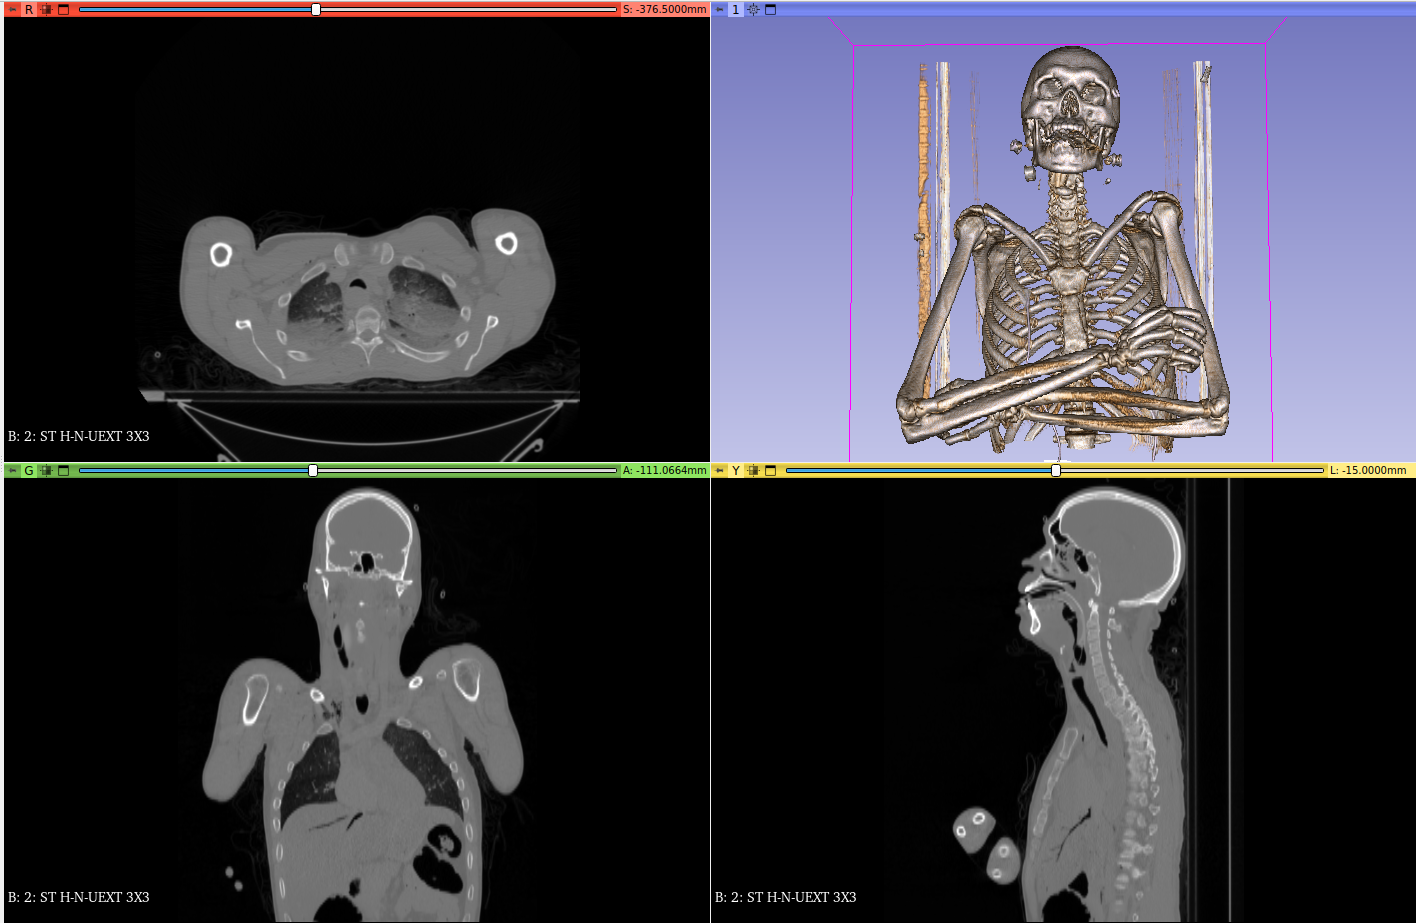
\includegraphics[width=0.8\textwidth]{imagenes/Chapter1/SlicerVisualization}
  \end{center}
  \caption{Ejemplo de visualización de un directorio \emph{DICOM}. Se pueden observar
  las proyecciones axial, coronal y sagital. Además de una renderización volumétrica
  de los huesos. Para ello se ha utilizado \emph{Slicer3D}~\cite{Slicer3D}}
  \label{fig:SlicerVisualization}
\end{figure}

A pesar de ello, las distorsiones, que son una ocurrencia común en las imágenes cotidianas, 
están muy presentes en las imágenes médicas~\cite{MedicalImpactOfDistortions}.
Prevalecen las distortiones de contraste, ruido y difuminado\footnotemark[3].
Estas a su vez, podrían afectar al volúmen 3D que se puede generar a partir 
las imágenes médicas. Y en medicina, 
se utilizan volúmenes tridimensionales, como tomografías computarizadas (TC) o 
resonancias magnéticas (RM) en lugar de radiografías convencionales, porque 
proporcionan una visión más completa y detallada de la anatomía y las estructuras 
internas del cuerpo, ver (\ref{fig:SlicerVisualization}). 
Esto brinda a los médicos una comprensión más completa de la anatomía y 
les ayuda a identificar con mayor precisión lesiones, enfermedades o anormalidades
\cite{3DImagingInMedicine, 3DImagingInMedicine2, ADAS3D}.

\footnotetext[3]{
  Con ruido nos referimos a pequeñas fluctuaciones no deseadas en los colores de 
  los píxeles debido a interferencias de todo tipo. Difuminado se refiere a la 
  pérdida de detalles en los bordes, como una pérdida de enfoque.
}
 
En~\cite{XrayRejectionFactor} se estudió las razones por las que se suelen 
rechazar las radiografías, la relación con la calidad de la imagen y el valor
del diagnóstico final. Reveló que la mayoría de los rechazos se producen por 
errores de posicionamiento, valores inadecuados de exposición, artefactos 
y los problemas de cooperación del paciente. 
Además, no es difícil imaginar que una alta 
calidad de imagen médica tiene implicaciones significativas sobre el cuidado
del paciente. Ya que la mala calidad de imagen puede provocar diagnósticos erróneos 
o falsos negativos. Sin mencionar los elevados costes que supone realizar 
nuevas pruebas para conciliar las anteriores.
 
Resolver este problema, o dar pasos hacia adelante, formulando una medida de calidad
puede conllevar a la mejora de los dispositivos médicos, de los algoritmos de comprensión, almacenado 
y transmisión de información. Tanto a nivel médico como cualquier 
aplicación con datos tridimensionales. Disminuyendo costes y ahorrando tiempo 
de consultas, mejorando la calidad de diagnóstico de pacientes. 

\section{Objetivos}
Para el desarrollo de este documento se plantean una serie de objetivos. 
El objetivo principal consiste en encontrar un método adecuado para atacar al 
problema de la estimación de la calidad de imágenes médicas tridimensionales. 
Este objetivo se puede descomponer en una serie de metas parciales: 
\begin{enumerate}
  \item Realizar una revisión del estado del arte para la estimación de calidad 
    de imágenes \emph{3D}. Comparativa entre métodos de aprendizaje automático 
    y de aprendizaje profundo. Estudiar el método o arquitectura más adecuada 
    para la resolución del problema y proponer posibles mejoras. 
  \item Estudiar las distorsiones comúnes en el mundo médico. 
    Dado que, actualmente, no existen conjuntos de datos disponibles para la 
    estimación de la calidad de imágenes médicas 3D, debemos analizar ejemplos 
    de conjuntos de datos genéricos disponibles y 
    seleccionar aquellos que traten las mismas distorsiones. 
  \item Preparar un conjunto de datos propio para validar. Preprocessar y 
    elegir las nubes de puntos iniciales de mejor calidad. 
    Estudiar la posibilidad de generar un \emph{pseudo-MOS} 
    utilizando métricas \emph{FR} del estado del arte actual o 
    realizar un experimento con un conjunto de individuos, 
    como consta en~\cite{ITU-R.2012, ITU-r.2021},
    para la obtención del \emph{MOS}. 
    Analizando a su vez las implicaciones de cada camino.
  \item Validar los resultados obtenidos, sacar conclusiones y propuestas 
    de cara al futuro.
\end{enumerate}
\section{Planificación del proyecto}
Al planificar el proyecto, es fundamental tener en cuenta que la asignatura del 
Trabajo Fin de Grado (TFG) tiene una carga de 12 créditos ECTS, donde cada 
crédito representa aproximadamente 25 horas de trabajo. 
En total, se estima que se necesitarán alrededor de 300 horas para llevar a cabo 
el proyecto. Considerando que el segundo cuatrimestre tiene aproximadamente 20 semanas, 
se requerirá dedicar al TFG unas 15 horas por semana, lo cual equivaldría a unas 3 horas 
diarias durante 5 días a la semana.
 
La naturaleza del proyecto no presenta una complejidad significativa en términos 
de su alcance y requisitos, lo cual permite abordar su desarrollo a través de un 
enfoque de ciclo de vida en cascada~\cite{ModeloEnCascada}. 
No obstante, bajo este enfoque se evita retroceder en cualquiera de las fases 
del ciclo, y aunque se espera que el diseño y los requisitos del sistema sean 
estables, existe la posibilidad de realizar ajustes menores conforme se obtenga
más información sobre el problema y los métodos. 
Es por ello que utilizamos una pequeña variante, la versión con retroalimentación.
 
Las fases del ciclo de vida son: 
\begin{itemize}
  \item Análisis de requisitos: Consiste en reuniones iniciales con los clientes, 
    en este caso sería los directores del TFG. Se organiza el análisis bibliográfico 
    del problema \emph{IQA} y \emph{PCQA}\footnotemark[4], teniendo en cuenta un estudio previo 
    de las distorsiones médicas.
  \item Diseño: Consistió en la investigación y selección de métodos conforme 
    al análisis anterior, tanto para la resolución como la validación de la solución. 
    Así como pruebas preliminares y diseño del software de experimentación. 
  \item Implementación: Consiste en la adaptación de las técnicas encontradas, 
    implementación de nuevas funcionalidas y generación de un conjunto de datos 
    médicos nuevos.
  \item Pruebas: Realización de diversos experimentos de validación, tanto al 
    la generación de las distorsiones como a los modelos y resultados.
\end{itemize}
\footnotetext[4]{\emph{Point cloud quality assessment} o estimación de calidad 
de nubes de puntos} 
\begin{table}[htp]
\centering
\resizebox{\textwidth}{!}{%
\begin{tabular}{|c|c|ll|llll|llll|lllll|llll|llll|}
\hline
\rowcolor[HTML]{FFC702} 
\cellcolor[HTML]{FFC702} & \cellcolor[HTML]{FFC702} & \multicolumn{2}{c|}{\cellcolor[HTML]{FFC702}\textbf{Febrero}} & \multicolumn{4}{c|}{\cellcolor[HTML]{FFC702}\textbf{Marzo}} & \multicolumn{4}{c|}{\cellcolor[HTML]{FFC702}\textbf{Abril}} & \multicolumn{5}{c|}{\cellcolor[HTML]{FFC702}\textbf{Mayo}} & \multicolumn{4}{c|}{\cellcolor[HTML]{FFC702}\textbf{Junio}} & \multicolumn{4}{c|}{\cellcolor[HTML]{FFC702}\textbf{Julio}} \\ \cline{3-25} 
\rowcolor[HTML]{FFC702} 
\multirow{-2}{*}{\cellcolor[HTML]{FFC702}\textbf{Tarea}} & \multirow{-2}{*}{\cellcolor[HTML]{FFC702}\begin{tabular}[c]{@{}c@{}}\textbf{Semanas -}\\ \textbf{Horas}\end{tabular}} & \multicolumn{1}{c}{\cellcolor[HTML]{FFC702}21} & \multicolumn{1}{c|}{\cellcolor[HTML]{FFC702}28} & \multicolumn{1}{c}{\cellcolor[HTML]{FFC702}07} & \multicolumn{1}{c}{\cellcolor[HTML]{FFC702}14} & \multicolumn{1}{c}{\cellcolor[HTML]{FFC702}21} & \multicolumn{1}{c|}{\cellcolor[HTML]{FFC702}28} & \multicolumn{1}{c}{\cellcolor[HTML]{FFC702}04} & \multicolumn{1}{c}{\cellcolor[HTML]{FFC702}11} & \multicolumn{1}{c}{\cellcolor[HTML]{FFC702}18} & \multicolumn{1}{c|}{\cellcolor[HTML]{FFC702}25} & \multicolumn{1}{c}{\cellcolor[HTML]{FFC702}02} & \multicolumn{1}{c}{\cellcolor[HTML]{FFC702}09} & \multicolumn{1}{c}{\cellcolor[HTML]{FFC702}16} & \multicolumn{1}{c}{\cellcolor[HTML]{FFC702}23} & \multicolumn{1}{c|}{\cellcolor[HTML]{FFC702}30} & \multicolumn{1}{c}{\cellcolor[HTML]{FFC702}06} & \multicolumn{1}{c}{\cellcolor[HTML]{FFC702}13} & \multicolumn{1}{c}{\cellcolor[HTML]{FFC702}20} & \multicolumn{1}{c|}{\cellcolor[HTML]{FFC702}27} & \multicolumn{1}{c}{\cellcolor[HTML]{FFC702}04} & \multicolumn{1}{c}{\cellcolor[HTML]{FFC702}11} & \multicolumn{1}{c}{\cellcolor[HTML]{FFC702}18} & \multicolumn{1}{c|}{\cellcolor[HTML]{FFC702}25} \\ \hline
Análisis de Requisitos & 4 - 60 & \cellcolor[HTML]{9B9B9B} & \cellcolor[HTML]{9B9B9B} & \cellcolor[HTML]{9B9B9B} & \cellcolor[HTML]{9B9B9B} & \cellcolor[HTML]{9B9B9B} &  &  &  &  &  &  &  &  &  &  &  &  &  &  &  &  &  &  \\ \cline{1-1}
Diseño & 4 - 60 &  &  &  &  & & \cellcolor[HTML]{9B9B9B} & \cellcolor[HTML]{9B9B9B} & \cellcolor[HTML]{9B9B9B} & \cellcolor[HTML]{9B9B9B}  & \cellcolor[HTML]{9B9B9B} &  &  &  &  &  &  &  &  &  &  &  &  &  \\ \cline{1-1}
Implementación & 6 - 90 &  &  &  &  &  &  &  &  & & & \cellcolor[HTML]{9B9B9B} & \cellcolor[HTML]{9B9B9B} & \cellcolor[HTML]{9B9B9B} & \cellcolor[HTML]{9B9B9B} & \cellcolor[HTML]{9B9B9B} &  &  &  &  &  &  &  &  \\ \cline{1-1}
Pruebas & 6 - 90 &  &  &  &  &  &  &  &  &  &  &  &  &  &  & & \cellcolor[HTML]{9B9B9B} & \cellcolor[HTML]{9B9B9B} & \cellcolor[HTML]{9B9B9B} & \cellcolor[HTML]{9B9B9B} & &  &  &  \\ \hline
\end{tabular}%
}
\caption{Planificación temporal inicial del proyecto}
\label{tab:PlanificacionTemporal}
\end{table}

La planificación (\ref{tab:PlanificacionTemporal}) se tomó como referencia, pero no de forma estricta. Ya que se 
tuvo en cuenta que el autor estaba realizando prácticas de empresa, tenía 
una asignatura y participaba de un curso de \emph{Google} ofrecido por la universidad.
Además, se esperaba que ocurriera retrasos sobre todo en la implementación, 
como se puede ver en (\ref{tab:PlanificacionFinal}), dado la novedad de la propuesta
y dificultad del problema. Un ejemplo fue a la hora de simular las distorsiones 
médicas, caso que fue algo iterativo y manual. 

\begin{table}[H]
\resizebox{\textwidth}{!}{%
\begin{tabular}{|c|c|ll|llll|llll|lllll|llll|llll|}
\hline
\rowcolor[HTML]{FFC702} 
\cellcolor[HTML]{FFC702} & \cellcolor[HTML]{FFC702} & \multicolumn{2}{c|}{\cellcolor[HTML]{FFC702}\textbf{Febrero}} & \multicolumn{4}{c|}{\cellcolor[HTML]{FFC702}\textbf{Marzo}} & \multicolumn{4}{c|}{\cellcolor[HTML]{FFC702}\textbf{Abril}} & \multicolumn{5}{c|}{\cellcolor[HTML]{FFC702}\textbf{Mayo}} & \multicolumn{4}{c|}{\cellcolor[HTML]{FFC702}\textbf{Junio}} & \multicolumn{4}{c|}{\cellcolor[HTML]{FFC702}\textbf{Julio}} \\ \cline{3-25} 
\rowcolor[HTML]{FFC702} 
\multirow{-2}{*}{\cellcolor[HTML]{FFC702}\textbf{Tarea}} & \multirow{-2}{*}{\cellcolor[HTML]{FFC702}\begin{tabular}[c]{@{}c@{}}\textbf{Semanas -}\\ \textbf{Horas}\end{tabular}} & \multicolumn{1}{c}{\cellcolor[HTML]{FFC702}21} & \multicolumn{1}{c|}{\cellcolor[HTML]{FFC702}28} & \multicolumn{1}{c}{\cellcolor[HTML]{FFC702}07} & \multicolumn{1}{c}{\cellcolor[HTML]{FFC702}14} & \multicolumn{1}{c}{\cellcolor[HTML]{FFC702}21} & \multicolumn{1}{c|}{\cellcolor[HTML]{FFC702}28} & \multicolumn{1}{c}{\cellcolor[HTML]{FFC702}04} & \multicolumn{1}{c}{\cellcolor[HTML]{FFC702}11} & \multicolumn{1}{c}{\cellcolor[HTML]{FFC702}18} & \multicolumn{1}{c|}{\cellcolor[HTML]{FFC702}25} & \multicolumn{1}{c}{\cellcolor[HTML]{FFC702}02} & \multicolumn{1}{c}{\cellcolor[HTML]{FFC702}09} & \multicolumn{1}{c}{\cellcolor[HTML]{FFC702}16} & \multicolumn{1}{c}{\cellcolor[HTML]{FFC702}23} & \multicolumn{1}{c|}{\cellcolor[HTML]{FFC702}30} & \multicolumn{1}{c}{\cellcolor[HTML]{FFC702}06} & \multicolumn{1}{c}{\cellcolor[HTML]{FFC702}13} & \multicolumn{1}{c}{\cellcolor[HTML]{FFC702}20} & \multicolumn{1}{c|}{\cellcolor[HTML]{FFC702}27} & \multicolumn{1}{c}{\cellcolor[HTML]{FFC702}04} & \multicolumn{1}{c}{\cellcolor[HTML]{FFC702}11} & \multicolumn{1}{c}{\cellcolor[HTML]{FFC702}18} & \multicolumn{1}{c|}{\cellcolor[HTML]{FFC702}25} \\ \hline
Análisis de Requisitos & 5 - 75 & \cellcolor[HTML]{9B9B9B} & \cellcolor[HTML]{9B9B9B} & \cellcolor[HTML]{9B9B9B} & \cellcolor[HTML]{9B9B9B} & &  &  &  &  &  &  &  &  &  &  &  &  &  &  &  &  &  &  \\ \cline{1-1}
Diseño & 4 - 60 &  &  &  &  & \cellcolor[HTML]{9B9B9B} & \cellcolor[HTML]{9B9B9B} & \cellcolor[HTML]{9B9B9B} & \cellcolor[HTML]{9B9B9B} & &  &  &  &  &  &  &  &  &  &  &  &  &  &  \\ \cline{1-1}
Implementación & 8 - 120 &  &  &  &  &  &  &  &  &  \cellcolor[HTML]{9B9B9B} & \cellcolor[HTML]{9B9B9B} & \cellcolor[HTML]{9B9B9B} & \cellcolor[HTML]{9B9B9B} & &  & \cellcolor[HTML]{9B9B9B}  & \cellcolor[HTML]{9B9B9B}  & & & \cellcolor[HTML]{9B9B9B} & \cellcolor[HTML]{9B9B9B} &  &  &  \\ \cline{1-1}
Pruebas & 5 - 75 &  &  &  &  &  &  &  &  &  &  &  &  & \cellcolor[HTML]{9B9B9B}   & \cellcolor[HTML]{9B9B9B} & & & \cellcolor[HTML]{9B9B9B} & \cellcolor[HTML]{9B9B9B} &  &  & \cellcolor[HTML]{9B9B9B} & \cellcolor[HTML]{9B9B9B} & \\ \hline
\end{tabular}%
}
\caption{Planificación resultante del proyecto}
\label{tab:PlanificacionFinal}
\end{table}

Para realizar este proyecto se tuvo en cuenta los siguientes materiales:
Suscripción a \emph{Google Colab Pro}, un pórtatil personal de gama media, 
\emph{Google Drive 100GB} y otros gastos. 
Además, para el coste estimado, se asume un salario de 25\officialeuro/hora, como para un investigador \emph{senior} o
responsable I+D de una empresa tecnológica en España. 
 
Respecto al servidor GPU, con las especificaciones actuales de \emph{Google}, 
se estima un coste aproximado de 10.000\officialeuro. Se asume una amortización de 2 años, 
lo que implica un pago diario de 13.70\officialeuro. El desglose total de los costes 
se puede ver en la siguiente tabla (\ref{tab:TotalGastos})

\begin{table}[htp]
\centering
\begin{tabular}{ll}
\hline
\multicolumn{1}{|l|}{\cellcolor[HTML]{FFCB2F}{Fecha inicio}} & \multicolumn{1}{l|}{21/02/2022} \\ \hline
\multicolumn{1}{|l|}{\cellcolor[HTML]{FFCB2F}{Fecha fin}} & \multicolumn{1}{l|}{25/07/2022} \\ \hline
\multicolumn{1}{|l|}{\cellcolor[HTML]{FFCB2F}{Duración}} & \multicolumn{1}{l|}{154 días, 110 laborables} \\ \hline
\textbf{} & 
\end{tabular}
\caption{Total de horas y días trabajados}
\label{tab:TotalTrabajado}
\end{table}
\begin{table}[htp] 
  \centering
  \begin{tabular}{ll}
\hline
\rowcolor[HTML]{FFCB2F} 
\multicolumn{1}{|c|}{\cellcolor[HTML]{FFCB2F}{Item}} & \multicolumn{1}{c|}{\cellcolor[HTML]{FFCB2F}{Costo}} \\ \hline
\multicolumn{1}{|l|}{Salario} & \multicolumn{1}{l|}{8 250.00\officialeuro} \\ \hline
\multicolumn{1}{|l|}{Portátil de Gama Media} & \multicolumn{1}{l|}{700.00\officialeuro} \\ \hline
\multicolumn{1}{|l|}{Google Colab Pro} & \multicolumn{1}{l|}{55.50\officialeuro} \\ \hline
\multicolumn{1}{|l|}{Servidor GPU} & \multicolumn{1}{l|}{2 109.8\officialeuro} \\ \hline
\multicolumn{1}{|l|}{Google Drive 100GB} & \multicolumn{1}{l|}{10.00\officialeuro} \\ \hline
\multicolumn{1}{|l|}{Otros} & \multicolumn{1}{l|}{300.00\officialeuro} \\ \hline
\multicolumn{1}{|r|}{\cellcolor[HTML]{FFCB2F}{Total}} & \multicolumn{1}{l|}{ 11 425.3 \officialeuro} \\ \hline
\textbf{} & 
\end{tabular}
\caption{Estimación final de coste del proyecto}
\label{tab:TotalGastos}
\end{table}
